\documentclass[14pt]{extarticle}
% \documentclass[14pt]{article}

% \usepackage[style=authoryear,maxbibnames=9,maxcitenames=2,uniquelist=false,backend=biber,doi=false,url=false]{biblatex}
% \addbibresource{$BIB} % bibtex location
% \renewcommand*{\nameyeardelim}{\addcomma\space} % have comma in parencite
\usepackage{natbib}

\usepackage{xcolor}
\usepackage{amsmath}
\newcommand{\tuple}[1]{ \langle #1 \rangle }
%\usepackage{automata}
\usepackage{times}
\usepackage{ltablex}
\usepackage{tasks}

%%%%%% Template
\usepackage{hyperref}
\hypersetup{colorlinks=true,allcolors=blue}

\usepackage{vmargin}
\setpapersize{USletter}
\setmarginsrb{1.0in}{1.0in}{1.0in}{0.6in}{0pt}{0pt}{0pt}{0.4in}

% HOW TO USE THE ABOVE:
%\setmarginsrb{leftmargin}{topmargin}{rightmargin}{bottommargin}{headheight}{headsep}{footheight}{footskip}
%\raggedbottom
% paragraphs indent & skip:
\parindent  0.3cm
\parskip    -0.01cm

\usepackage{tikz}
\usetikzlibrary{backgrounds}

% hyphenation:
\hyphenpenalty=10000 % no hyphen
% \exhyphenpenalty=10000 % no hyphen
% \sloppy

% notes-style paragraph spacing and indentation:
\usepackage{parskip}
\setlength{\parindent}{0cm}

% let derivations break across pages
\allowdisplaybreaks

\newcommand{\orange}[1]{\textcolor{orange}{#1}}
\newcommand{\blue}[1]{\textcolor{blue}{#1}}
\newcommand{\red}[1]{\textcolor{red}{#1}}
\newcommand{\freq}[1]{{\bf \sf F}(#1)}
\newcommand{\datafreq}[2]{{{\bf \sf F}_{#1}(#2)}}

\def\qqquad{\quad\qquad}
\def\qqqquad{\qquad\qquad}

%%%%%%%%%%%%%%%%%%%%%%%%%%%%%%%%%%%%%%%%%%%%%%%%%%%%%%%%%%%%%%%%%%%%%%%%%%%%%%%%
%%%%%%%%%%%%%%%%%%%%%%%%%%%%%%%%%%%%%%%%%%%%%%%%%%%%%%%%%%%%%%%%%%%%%%%%%%%%%%%%

% fill-in-blank question style, found in https://tex.stackexchange.com/a/505089

\usepackage{ifthen}
\usepackage{tocloft}
\usepackage{exercise}
% \usepackage{xcolor}

% Set the Show Answers Boolean
\newboolean{showAns}
\setboolean{showAns}{false}
\newcommand{\showAns}{\setboolean{showAns}{true}}

% The length of the Answer line
\newlength{\answerlength}
\newcommand{\anslen}[1]{\settowidth{\answerlength}{#1}}

% ans command that indicates space for an answer or shows the answer in red
\newcommand{\ans}[1]{\settowidth{\answerlength}{\hspace{2ex}#1\hspace{2ex}}%
    \ifthenelse{\boolean{showAns}}%
        {\textcolor{red}{\underline{\hspace{2ex}#1\hspace{2ex}}}}%
        {\underline{\hspace{\answerlength}}}}%

\newcommand{\details}[1]{\settowidth{\answerlength}{#1}%
    \ifthenelse{\boolean{showAns}}%
        {\\ \textcolor{blue}{#1}}%
        {}}%

% Formatting how multiple choices Questions are formated.
\settasks{label=(\Alph*), label-width=30pt}


% Some commands for the Exercise Question package
\renewcommand{\QuestionNB}{\Large\protect\textcircled{\small\bfseries\arabic{Question}}\ }
\renewcommand{\ExerciseHeader}{} %no header
\renewcommand{\QuestionBefore}{3ex} %Space above each Q
\setlength{\QuestionIndent}{8pt} % Indent after Q number


% To create the list of answers with tocloft...
\newcommand{\listanswername}{Answers}
\newlistof[Question]{answer}{Answers}{\listanswername}

% Creates a TOC for Answers
\newcounter{prevQ}
\newcommand{\answer}[1]{\refstepcounter{answer}%
\ans{#1}%
\ifnum\theQuestion=\theprevQ%
        \addcontentsline{Answers}{answer}{\protect\numberline{}#1}% don't include the Q number
        \else%
        \addcontentsline{Answers}{answer}{\protect\numberline{\theQuestion}#1}%
        \setcounter{prevQ}{\value{Question}}%
        \fi%
        }%

% \hyphenpenalty=10000 % no hyphen
% \exhyphenpenalty=10000 % no hyphen
\sloppy              % hyphen

\newcommand{\HRule}{\rule{\linewidth}{0.5mm}}
\newcommand{\Hrule}{\rule{\linewidth}{0.3mm}}

%tocloft formatting listofanswers
\renewcommand{\cftAnswerstitlefont}{\bfseries\large}
\renewcommand{\cftanswerdotsep}{\cftnodots}
\cftpagenumbersoff{answer}
\addtolength{\cftanswernumwidth}{10pt}

\makeatletter% since there's an at-sign (@) in the command name
\renewcommand{\@maketitle}{%
  \parindent=0pt% don't indent paragraphs in the title block
  \centering
  {\LARGE \bfseries \@title} \\
  \vspace{5pt}
  {\large \textit{\@author}} \\
  \HRule \\
  % \vspace{1em}
}
\makeatother% resets the meaning of the at-sign (@)

\title{ECON 2002.01 Problem Set 2 }
\author{Unit 3 \\
  \vspace{5pt}
    Hui-Jun Chen}


%%%%%%%%%%%%%%%%%%%%%%%%%%%%%%%%%%%%%%%%%%%%%%%%%%%%%%%%%%%%%%%%%%%%%%%%%%%%%%%%
%%%%%%%%%%%%%%%%%%%%%%%%%%%%%%%%%%%%%%%%%%%%%%%%%%%%%%%%%%%%%%%%%%%%%%%%%%%%%%%%
\begin{document}

\maketitle
\showAns
\listofanswer

\begin{Exercise}

\Question (OUP-U3-Q1) You currently work for 40 hours a week at wage rate of £12 an hour. Your free hours are defined as the number of hours not in work, which in this case is 24 hours × 7 days – 40 hours = 128 hours per week. Suppose that you are happy to keep your total weekly income constant. Then:
\answer{B}
\begin{tasks}(1)
    \task If your wage rate increases to £16 an hour, then your free time will increase by 6\%.
        \details{The current total weekly income is £12 × 40 hours = £480. At the wage rate of £16, you will only need to work for 480 /16 = 30 hours a week. This will increase your free time to 138 hours, which is an increase of (138 – 128) / 128 = 7.8\%.}
    \task To have 12.5\% more free time, your wage rate needs to increase by £8.
        \details{The current total weekly income is £12 × 40 hours = £480. 12.5\% extra free time means 128 hours × 1.125 = 144 hours of free time, or 24 hours of work. To keep your weekly income constant, your wage rate needs to increase to £480 / 24 = £20 an hour, which is an increase of £8.}
    \task Doubling the wage rate would decrease your working hours by a third.
        \details{The current total weekly income is £12 × 40 hours = £480. If the wage rate doubles to £24, your working hours fall to 480 /24 = 20 hours a week, i.e. it halves.}
    \task A wage cut of 25\% leaves you with only 100 hours of free time.
        \details{The current total weekly income is £12 × 40 hours = £480. A wage cut of 25\% means your new hourly wage is £12 × (1 – 0.25) = £9. To keep the weekly income constant you will have to work 480 ÷ 9 = 53 hours and 20 minutes, which leaves you with 114 hours and 40 minutes of free time.}
\end{tasks}

\Question (OUP-U3-Q4) The following is a plot of GDP per capita against average annual hours of free time per worker in different countries. Which of the following statements is correct?
\answer{A}
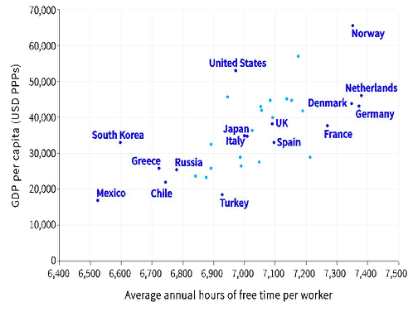
\includegraphics[width=\textwidth]{../QuestionBankImage/OUP-U3-Q4-01.png}
\begin{tasks}(1)
    \task Workers in the US and Turkey enjoy a similar amount of free time despite the huge disparity of income.
        \details{This is evident in the diagram: workers from the US and Turkey both enjoy 6900-7000 hours of free time but the US has a much higher GDP per capita than Turkey.}
    \task Japanese workers require more hours of work to produce the same level of output per capita as Korean workers.
        \details{The converse is true; Japanese workers have more free time than Korean workers have, but produce similar output per capita.}
    \task If German workers worked as many hours as the Norwegians, then they will be able to produce a similar level of output per capita.
        \details{The Norwegians produce higher output per capita than the Germans, despite both working a similar number of hours.}
    \task The plot gives strong evidence that workers choose to enjoy more free time as their living standards rise.
        \details{While there is positive correlation between GDP per capita and free time, the dispersion suggests that for some nationalities the increase in living standard takes the form of more goods and services to consume (e.g. the US), while for others this has taken the form of more leisure time (e.g. France).}
\end{tasks}

\Question (OUP-U3-Q9) The figure shows the indifference curves of a student for the two ‘goods’, free time and final grade. Based on this information, which of the following statements is correct?
\answer{A}
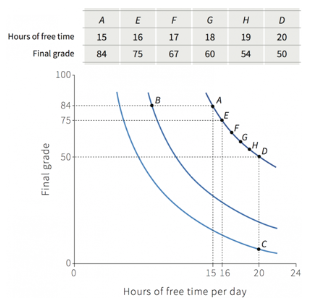
\includegraphics[width=\textwidth]{../QuestionBankImage/OUP-U3-Q9-01.png}
\begin{tasks}(1)
    \task At A, the student is willing to give up 34 grade points for five extra hours of free time.
        \details{This is true, as points A and D are on the same indifference curve.}
    \task A is the student’s most preferred choice as she would be attaining the highest grade.
        \details{The student is indifferent between A and all the other points on the same indifference curve i.e. E, F, G, H, and D.}
    \task The student strictly prefers a grade of 54 with 19 hours of free time to a grade of 67 with 18 hours of free time.
        \details{A grade of 54 with 19 hours of free time is point H. The student is indifferent between this point and point F, where she gets a grade of 67 with 17 hours of free time. She would therefore strictly prefer a grade of 67 with 18 hours of free time to H.}
    \task If at B the number of free hours is 10, then the student is 50\% happier at A than at B.
        \details{Higher indifference curves imply higher levels of utility, but the specific level of utility depends on the student’s relative preferences for both goods. It is not necessarily true that 50\% additional free time would make the student 50\% happier.}
\end{tasks}

\Question (OUP-U3-Q14) You have two choices for how you are going to spend Saturday evening. You can go to the pub with your friends, which will cost you £30 for the evening. The pleasure you anticipate from this experience is worth £50 to you. Or you can go to the theatre. The ticket will cost you £50, but you value the experience at £60. Based on this information, which of the following statements is correct?
\answer{C}
\begin{tasks}(1)
    \task The opportunity cost of an evening at the theatre is £10.
        \details{The opportunity cost of an evening at the theatre is the economic rent of the alternative, which is going to the pub. This is £50 – £30 = £20.}
    \task The economic cost of going to the theatre is £60.
        \details{The economic cost of going to the theatre is the sum of the accounting cost and the opportunity cost, which in this case is £50 + £20 = £70.}
    \task The economic rent of going to the theatre is -£10.
        \details{The economic rent is the difference between the value of the experience and its economic cost, which here is £60 – £70 = -£10.}
    \task Based on economic rent alone, you would choose to go to the theatre.
        \details{The economic rent for the theatre is negative at -£10, whereas the economic rent for the pub is positive at £10. Therefore you would choose to go to the pub instead of the theatre.}
\end{tasks}

\Question (OUP-U3-Q18) The figure shows a student’s feasible frontier and her indifference curves for final exam marks and the hours of free time per day. The table also gives the marginal rate of substitution (MRS) and the marginal rate of transformation (MRT) for the points shown in the figure. Based on this information, which of the following statements is correct?
\answer{A}
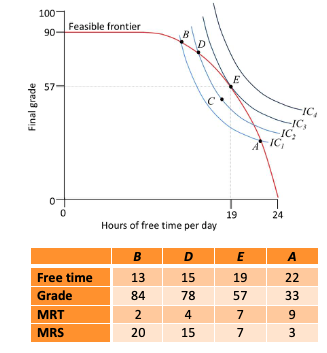
\includegraphics[width=\textwidth]{../QuestionBankImage/OUP-U3-Q18-01.png}

\begin{tasks}(1)
    \task At A, one hour of free time is equivalent in value to 3 grade points. However, 1 extra hour of studying leads to 9 extra grade points. She should therefore study more.
        \details{This is case where MRT > MRS.}
    \task At B, one hour of free time is equivalent in value to 2 grade points. However, 1 extra hour of studying leads to 20 extra grade points. She should therefore study more.
        \details{The statement has MRT and MRS the wrong way round.}
    \task At D, the MRT of 4 means that if she gives up all of her free time, she can attain 60 extra grade points.
        \details{The MRT changes along the curve. In particular, the feasible frontier flattens for lower hours of free time, suggesting that the MRT becomes zero (i.e. no gain from extra hours of studying) past a certain number of hours studied.}
    \task 	At E, the MRS matches the student’s MRT. Therefore she should exchange one hour of free time with 7 extra grade points.
        \details{MRS = MRT means that the student has no incentive to either increase or decrease the amount of free time consumed}
\end{tasks}

\Question (OUP-U3-Q23) Consider a worker whose choice is between hours of free time and consumption. His company has now cut his wage rate. Which of the following statements is correct?
\answer{C}
\begin{tasks}(1)
    \task As a result of the substitution effect, the worker would reduce his free time.
        \details{A wage cut implies a fall in the opportunity cost of free time. Therefore the worker would increase his free time as a result of the substitution effect.}
    \task The income effect means that the worker would increase his free time.
        \details{The worker’s total income will fall as a result of the wage cut. This implies a negative income effect.}
    \task The worker may or may not reduce his free time as a result of the wage cut.
        \details{The worker will increase his free time if the positive substitution effect dominates the negative income effect. On the other hand, if the income effect dominates the substitution effect, then he will reduce his free time.}
    \task The income effect will always dominate the substitution effect of the wage cut.
        \details{Whether the income effect dominates the substitution effect or not depends on the shape of the worker’s indifference curves.}
\end{tasks}

\Question (TEA-U3-Q5) Consider indifference curves for the consumption of milk and chocolates (you may assume that both are 'goods'). The indifference curves are drawn with the number of chocolate bars on the horizontal axis and pints of milk on the vertical axis. Suppose that at every point, consumer A's indifference curve is flatter than consumer B's. In this case, we can conclude that:
\answer{D}
\begin{tasks}(1)
    \task Consumer A's utility from chocolate is higher than Consumer B's.
        \details{Utility is an ordinal concept (increasing transformations of a utility function represent the same preferences between milk and chocolate), so utility levels cannot be compared across consumers.}
    \task The price of milk relative to the price of chocolates is higher for consumer A than for consumer B.
        \details{The relative price affects the point chosen on the indifference curves, but does not depend on their slope. Usually the prices of goods are taken as given (all shoppers in a particular supermarket face the same prices).}
    \task Consumer A's indifference curves cannot cross/intersect Consumer B's indifference curves.
        \details{The indifference curves of a particular consumer cannot cross. The indifference curves of consumers with different preferences can cross.}
    \task Given the same amount of chocolates, consumer A is willing to swap one bar of chocolate for a smaller amount of milk than consumer B.
        \details{In this case, a flatter indifference curve means that consumer A has a stronger preference for milk over chocolate compared to consumer B, and so is willing to accept a smaller amount of milk for the same amount of chocolate.}
\end{tasks}

\Question (UCL-J18-Q2) Which (if any) of the following statements regarding hours of work and income must be true, based only on the information given? Note: a normal good is one for which demand rises with income.
\answer{C}
\begin{tasks}(1)
    \task The opportunity cost of an hour reading the newspaper is the hourly wage rate.
        \details{The opportunity cost is the net utility from the next-best alternative. This statement is only true if the next-best alternative is to work, and the hourly rate is the same as your net utility (you may have disutility from working, so net utility will be lower than the hourly rate).}
    \task France must have a higher average wage than the US, as the French work less hours than the Americans.
        \details{This statement is not necessarily true - people in France may have different preferences from people in the US, so may choose to work different hours for the same wage rate. We therefore cannot infer that working less hours means the wage rate is definitely higher in France.}
    \task An unconditional cash transfer to citizens would encourage them to work less if leisure is a normal good.
        \details{The cash transfer has a positive income effect and no substitution effect (relative prices do not change), so the overall effect is to increase leisure. }
    \task An unexpected wage increase will always motivate citizens to work more.
        \details{We need to evaluate the amount of income and substitution effects to determine the impact of wage increase on hours of work.}
\end{tasks}

\Question (ECO-U3-Q4) Figure 3.6 shows Alexei’s indifference curves for free time and final grade. Which of the following is true?
\answer{B}
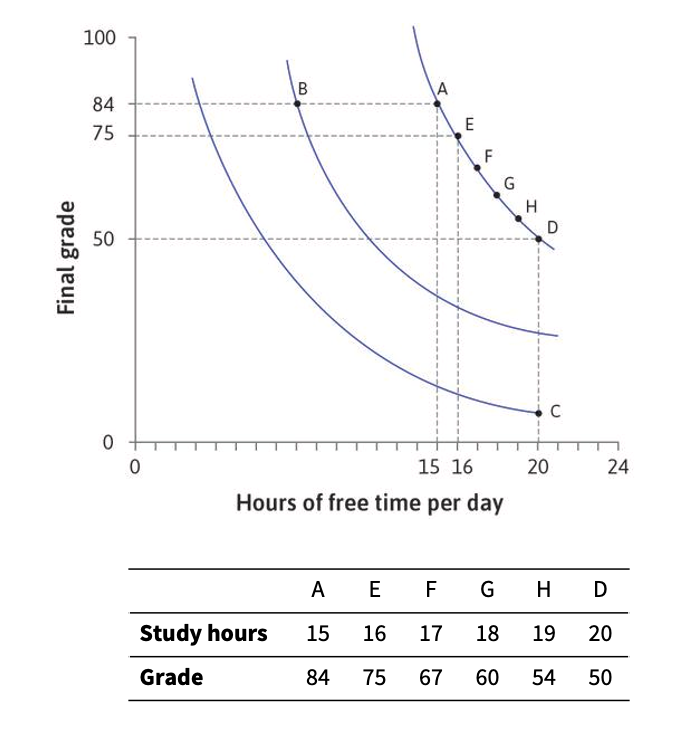
\includegraphics[width=\textwidth]{../QuestionBankImage/ECO-U3-Q4-01.png}
\begin{tasks}(1)
    \task Alexei prefers C to B because at C he has more free time.
        \details{The indifference curve through C is lower than that through B. Hence Alexei prefers B to C.}
    \task Alexei is indifferent between the grade of 84 with 15 hours of free time, and the grade of 50 with 20 hours of free time.
        \details{A, where Alexei has the grade of 84 and 15 hours of free time, and D, where Alexei has the grade of 50 with 20 hours of free time, are on the same indifference curve.}
    \task Alexei prefers D to C, because at D he has the same grade and more free time.
        \details{At D Alexei has the same amount of free time but a higher grade.}
    \task At G, Alexei is willing to give up 2 hours of free time for 10 extra grade points.
        \details{The opposite trade-off is true: going from G to D, Alexei is willing to give up 10 grade points for 2 extra hours of free time. Going from G to E, he is willing to give up 2 hours of free time for 15 extra grade points.}
\end{tasks}

\Question (OUP-U3-Q15) The following diagram is the feasible set of a student, showing the combinations of her final grade and the hours of free time per day. Based on this information, we can say that:
\answer{D}
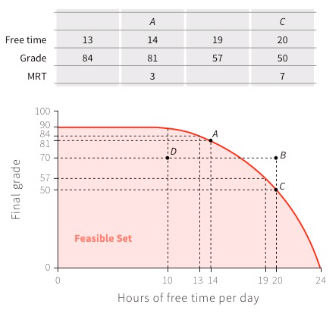
\includegraphics[width=\textwidth]{../QuestionBankImage/OUP-U3-Q15-01.png}
\begin{tasks}(1)
    \task Whether the student would choose A or B depends on her preferences.
        \details{B is outside the feasible set and therefore can never be chosen.}
    \task At A, the student can attain grade of 81 for 14 hours of study.
        \details{At A, the student is able to attain a grade of 81 and have 14 hours of free time, so she studies for 10 hours.}
    \task C would never be chosen over A.
        \details{The student can choose C over A if her indifference curves are steep enough.}
    \task The marginal rate of transformation increases with higher number of free hours.
        \details{For a higher number of free hours, sacrificing one hour of free time gives a larger increase in grade points.}
\end{tasks}

\end{Exercise}

\end{document}
